\chapter{Resultados}

\section{Reacciones de combustión y requerimiento de aire}
\par Al ejecutar el cálculo de combustión con los datos de composición de combustible y condiciones ambientales de las las Tablas \ref{tbl:combustible} y \ref{tbl:aire}, se obtuvieron los resultados mostrados en la Tabla \ref{tbl:combustion-data}. Adicionalmente, se generaron las composiciones molar y másica de los gases de combustión mostradas en la Tabla \ref{tbl:combustion-gas}.
\begin{table}[hbt] \begin{center}
\caption[Combustión simulada]{Combustión simulada.}
\label{tbl:combustion-data} \begin{tabular}{l|c}
	A/C másica teórica requerido					& 15,574 \\
	A/C másica húmeda con exceso de aire			& 18,689 \\
	Relación de gases de combustión por unidad de aire& 19,689 \\
	Poder Calorífico Neto  (NCV), kJ/kg				& 45.718,6 \\
	Poder Calorífico Bruto (GCV), kJ/kg				& 50.268,0 \\
	Peso Molecular (PM) del combustible, kg/kmol	& 21,149 \\
	PM de los gases de combustión, kg/kmol				& 27,911 \\
\end{tabular} \end{center} \end{table}
\begin{table}[htb] \begin{center}
\caption[Composición de los gases de combustión]
{Composición porcentual de los gases de combustión.}
\label{tbl:combustion-gas} \begin{tabular}{l|c|c|c}
	   & \% Peso & \% Moles \\
	\hline
	Nitrógeno ($N_2$)			& 72,121	& 71,860 \\
	Oxígeno ($O_2$)				& 3,636 	& 3,172	 \\
	Dióxido de carbono ($CO_2$)	& 13,753	& 8,723	 \\
	Vapor de agua ($H_2O$)		& 10,490	& 16,245 \\
	Dióxido de azufre ($SO_2$)	& 0,000 	& 0,000	 \\
\end{tabular} \end{center} \end{table}

\par Para validar la confiabilidad de estos resultados del simulador se compararon con los obtenidos empleando el software comercial WinHeat\copyright\ para el diseño y evaluación de hornos, propiedad de Esteem Projects Pvt. Ltd., con una licencia autorizada para la versión 3.0. La conclusión de esta comparación arrojó que la diferencia entre los resultados de ambos simuladores para el cálculo de la combustión es menor a 0,1\%. 
\section{Simulación térmica del horno}
\par Los datos específicos del fluido y condiciones de operación que quedan por definir se muestran en la siguiente Tabla \ref{tbl:props}:
\begin{table}[htb]\begin{center}
\caption[Datos del fluido y condiciones de operación]{Datos del fluido y condiciones de operación}
\label{tbl:props}\begin{tabular}{l|c|c}
	Flujo del residuo atmosférico a calentar  & \multicolumn{2}{c}{12.019,6 toneladas/día} \\
	\hline
    Propiedades del residuo  & Entrada   & Salida \\
    Temperatura          (°C)       & 359    & 411 \\
	Viscosidad	         (cp)	    & 1,45	& 0,96 \\
	Capacidad calorífica (kJ/kg°C)	& 2,83 	& 2,943	 \\
	Conductividad térmica (kJ/h m²°C) & 0,230& 0,235	 \\
	\hline
	Factores de ensuciamiento & Interno & Externo\\
	Sección radiante	(m²°C/W)  & 0,000176	& 0,0 \\
	Sección escudo		(m²°C/W)  & 0,000176	& 0,0 \\
	Sección convectiva	(m²°C/W)  & 0,000176	& 0,0 \\
    \hline
	Pérdidas de calor por paredes al ambiente & \multicolumn{2}{c}{1,5\%} \\
\end{tabular}\end{center}\end{table}
\par Los resultados de de los balances de energía por sección correspondientes a las ecuaciones \ref{eq:rad}, \ref{eq:esc} y \ref{eq:conv}, del modelo descrito en comparación con los resultados del simulador WinHeat\copyright, se muestran en las Tablas \ref{tbl:compara-zr}, \ref{tbl:compara-ze} y \ref{tbl:compara-zc}.
\par En estas tablas se pueden apreciar las diferencias dentro de cada sección entre ambos simuladores, se observa que la diferencia máxima en las distribuciones de calor por zona es de 2,5\%, esto atado a diferencias en las temperaturas de entrada y salida, en las secciones internas, de los gases de combustión y del fluido de proceso.
\par Los resultados que mostraron diferencias significativas fueron corroborados manualmente con las ecuaciones correspondientes. Al comprobar estos valores en los rangos de diseño del horno, se cierra la aproximación del calor absorbido por el fluido con una tolerancia menor al 0,5\%, considerando de esta forma que el algoritmo funciona correctamente.

\subsection{Validación de la sección radiante}
\begin{table}[H] \begin{center}
\caption[Resultados en zona radiante]{Comparación de resultados de la zona radiante.}
\label{tbl:compara-zr} \begin{tabular}{l|c|c}
	& Simulador & WinHeat\copyright \\
Temperatura de entrada del residuo, °C	& 379 & 378	\\
Temperatura de salida del residuo, °C	& 411 & 411	\\
Temperatura de pared de tubos, °C	    & 432 & 459	\\
Temperatura de arco radiante, °C        & 798 & 813	\\
\hline
Calor suministrado por el combustible, MW	& 26,235 & 25,790	\\
Calor sensible del aire atmosférico, MW		& 0,123 & 0,119	\\
Calor sensible del combustible, MW			& 0,022 & 0,000	\\
\hline
Calor de gases de combustión, MW		    & 11,084 & 10,615	\\
Pérdidas de calor al ambiente, MW	        & 0,394 & 0,226	\\
Calor radiante transferido al escudo, MW	& 1,747 & 1,665	\\
Calor convectivo transferido al residuo, MW	& 1,705 & 1,650	\\
Calor radiante transferido al residuo, MW	& 11,444 & 11,753	\\
Calor absorbido por el residuo, MW	        & 13,155 & 13,417	\\
\hline
Distribución de calor en zona radiante, \%	& 62,78 & 64,01 \\
\hline
Área total del banco de tubos ($A_t$), m$^2$& 547,09 & 547,01 \\
Área refractaria ($Ar$), m$^2$		    & 566,42 & 541,70 \\
Área de plano frontal ($Acp$), m$^2$	& 323,05 & 369,73 \\
Factor de efectividad alfa			    & 0,904 & 0,904 \\
\hline
Coef. de convección int., ($h_i$) kJ/h-m$^2$-C	& 2.770,4 & 2.992,7 \\
Coef. de convección ext., ($h_c$) kJ/h-m$^2$-C	& 30,663 & no reportado \\
\hline
Longitud media del haz radiante, ft	& 20,829 & 20,45 \\
P$_{CO_2}$+P$_{H_2O}$, atm 		    & 0,249 & 0,250 \\
\end{tabular} \end{center} \end{table}
\par El área total de la superficie de los tubos es prácticamente idéntica, el número total de tubos y el espaciado es igual, contrariamente el área de plano frontal difiere en 12,6\%, lo que indica el uso de una ecuación distinta para $Acp$ por el simulador Winheat\copyright. Esto se refleja en la disminución de 2,77\% del calor cedido en esta zona al residuo atmosférico.

\subsection{Validación en la sección de escudo}
\par En esta sección la variación de temperatura del residuo concuerda entre ambos simuladores, con una diferencia no mayor a 0,1\%, en cambio la diferencia en la temperatura de los gases de combustión incrementa, haciendo que la diferencia de temperatura media logarítmica aumente significativamente.
\par Esto se puede atribuir a un mayor coeficiente de transferencia global convectiva reportado por Winheat\copyright, ya que el coeficiente de convección interno es aproximadamente igual en ambos simuladores la diferencia proviene del coeficiente de convección externo que no es reportado por el simulador de referencia.
\begin{table}[H] \begin{center}
\caption[Resultados de la zona escudo]{Comparación de resultados de la zona escudo.}
\label{tbl:compara-ze} \begin{tabular}{l|c|c}
	& Simulador & WinHeat\copyright \\
Temperatura de entrada del residuo, °C	& 370 & 369	\\
Temperatura de salida del residuo, °C	& 379 & 378	\\
Temperatura de pared de tubo, °C		& 401 & 407	\\
Temperatura de entrada de gases de combustión, °C	& 798 & 813	\\
Temperatura de salida de gases de combustión, °C	& 695 & 674	\\
Diferencia de temperatura media logarítmica, K	& 370 & 660 \\
\hline
Flujo de gases de combustión, kg/s	& 11,298 & 11,099	\\
Calor de gases de combustión, MW	& 1,587 & no reporta \\
Calor convectivo transferido, MW	& 1,586 & 1,957	\\
Calor radiante transferido, MW		& 1,747 & 1,665	\\
Calor absorbido por el fluido, MW	& 3,334 & 3,621	\\
Distribución de calor en zona escudo, \%& 15,86 &  17,3 \\
\hline
Área total de tubos de escudo ($A_t$), m$^2$& 154,688 & 158,678 \\
Área de plano frontal ($Acp$), m$^2$	   & 44,593 & no reporta \\
Factor de efectividad alfa			       & 1,00 & 1,00 \\
\hline
Coef. de transferencia global ($U_0$), kJ/h-m$^2$-C	& 100,253  & 121,016 \\
Coef. de convección interno, ($h_i$) kJ/h-m$^2$-C	& 4.426,5 & 4.411,3 \\
Coef. de convección externo, ($h_c$) kJ/h-m$^2$-C	& 30,663 & no reporta \\
\end{tabular} \end{center} \end{table}

\subsection{Validación de la sección convectiva}
\par La temperatura de chimenea, a la cual salen los gases de combustión del horno, es 9 °C mayor en el simulador desarrollado (2,3\%), lo que repercute en los valores de eficiencia obtenidos.
\begin{table}[H] \begin{center}
\caption[Resultados en zona convectiva]
{Comparación de resultados de la zona convectiva.}
\label{tbl:compara-zc} \begin{tabular}{l|c|c}
	& Simulador & WinHeat\copyright \\
Temperatura de entrada del residuo, °C		& 359 & 359	\\
Temperatura de salida del residuo, °C		& 370 & 369	\\
Temperatura de pared de tubo, °C		    & 366 & 361	\\
Temperatura de entrada de gases de combustión, °C	& 695 & 674	\\
Temperatura de salida de gases de combustión, °C	& 391 & 382	\\
Temperatura promedio de aletas, °C          & 366 & 364\\
Diferencia de temperatura media logarítmica, K	& 126 & 92 \\
\hline
Calor contenido en los gasaes, MW   & 4,457 & no reporta \\
Calor convección transferido, MW	& 4,465 & 3,998	\\
Calor absorbido por el fluido, MW	& 4,464 & 3,939	\\
Distribución de calor en zona convectiva, \%& 21,31 &  18,79 \\
\hline
Área total de tubos con aletas ($A_t$), m$^2$& 4.670,8 & 4.872,6 \\
Eficiencia de aletas, \%			& 98,77 & no reporta \\
\hline
Coef. tran. global ($U_0$), kJ/h-m$^2$-C	& 27,295 & 26,493 \\
Coef. de convección int., ($h_i$) kJ/h-m$^2$-C	& 4.300,2 & 4.331,4 \\
Coef. de convección ext., ($h_c$) kJ/h-m$^2$-C	& 26,261 & no reporta \\
Coef. externo promedio, ($h_p$) kJ/h-m$^2$-C	& 27,887 & 35,009 \\
Coef. externo efectivo, ($h_e$) kJ/h-m$^2$-C	& 27,563 & 30,689 \\
Coef. de radiación, ($h_r$) kJ/h-m$^2$-C	& 1,626  & no reporta \\
\end{tabular} \end{center} \end{table}
\par Las áreas de transferencia totales de los tubos del horno son iguales en la sección de radiación, 2,5\% menores en la sección de escudo y 4,1\% menores en la sección de convección, donde se incluye el área de las aletas; esto debido a posibles diferencias en las ecuaciones usadas por WinHeat\copyright, las cuales no son descritas en el programa o el manual de uso.
\par Por último, con mayor diferencia observada, se encuentran los coeficientes de transferencia de calor; en la zona radiante el único reportado por WinHeat\copyright \ es el coeficiente de convección interno que difiere en 7,1\%, en las otras zonas esta diferencia no supera 0,5\%; mientras que el coeficiente de transferencia global de la zona de escudo y convección difieren en 17,3\% y 4,2\% respectivamente.

\subsection{Resultados globales}
\par El flujo másico de combustible obtenido es ligeramente mayor (1,77\%) al reportado por el simulador de referencia, y la máxima diferencia en las temperaturas internas corresponde a la entrada del gas en la zona convectiva (2,97\%).
\par En adición a los resultados generados por el software WinHeat©, el simulador desarrollado muestra, en la Tabla \ref{tbl:compara-global}, los valores de emisiones de dióxido de carbono en toneladas/año, el calor liberado a la atmósfera con los gases de combustión y las eficiencias térmicas con base en los poderes caloríficos neto (NCV) y bruto (GCV)\cite{bib:api560}.
\begin{table}[H]\begin{center}
\caption[Resultados globales de la simulación]{Resultados globales de la simulación.}
\label{tbl:compara-global} \begin{tabular}{l|c|c}
	& Simulador & WinHeat\copyright \\
Flujo de combustible, kg/s		            & 0,574 & 0,564	\\
Calor liberado en chimenea, MW	    & 4,910 & no reporta \\
Eficiencia térmica del horno (NCV), \%	& 79,89  & 80,91 \\
Eficiencia térmica del horno (GCV), \%	& 72,70  & no reporta \\
Emisiones de CO$_2$ al ambiente, toneladas/año	& 49,006  & no reporta \\
\end{tabular} \end{center} \end{table}

\section{Curvas de tendencia}
\par Estas curvas son definidas dentro del rango de aplicación, muestran la confiabilidad (tendencias continuas y sin inestabilidades) del algoritmo y pueden ser usadas de manera educacional para observar el comportamiento de las variables operacionales del equipo.
\par Se obtienen al ejecutar la simulación seleccionando uno entre cuatro variables de entrada, ver Fig. \ref{fig:curvas}. Las variables escogidas fueron:
\begin{enumerate}
    \item El flujo de residuo.
    \item La temperatura de salida del residuo.
    \item El exceso de aire de combustión.
    \item La humedad relativa en el aire de combustión.
\end{enumerate}
\begin{figure}[H]\begin{center}
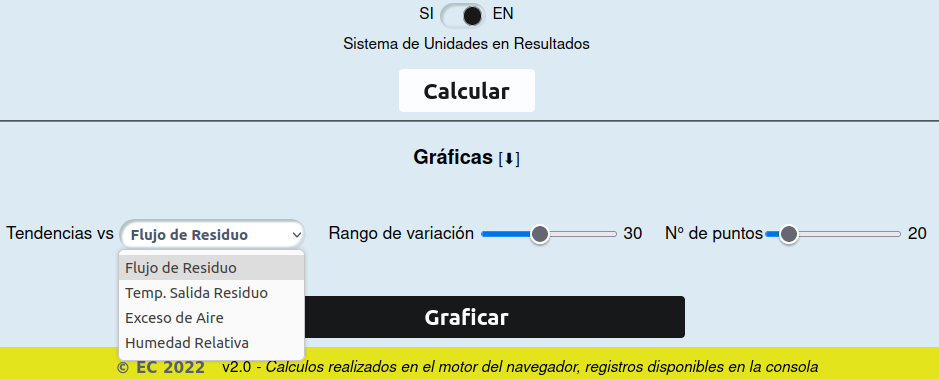
\includegraphics[scale=0.48]{images/curvas}
\caption[Opciones disponibles para graficar en el simulador]{Opciones disponibles para graficar en el simulador.}
\label{fig:curvas}\end{center}\end{figure}
\par Dependiendo del número de puntos escogidos por el usuario, el simulador podrá requerir más tiempo para finalizar los cálculos, en los rangos permitidos de la interfaz.
\par Definido un rango, este se divide entre un número de puntos establecido y se corre la simulación moviendo la variable escogida por cada punto.
\par Para observar y analizar los cambios generados se seleccionaron seis variables calculadas, a saber:
\begin{enumerate}
    \item El flujo de combustible.
    \item La temperatura de arco radiante.
    \item La temperatura de chimenea.
    \item La relación de absorción de calor entre las zona radiante y convectiva.
    \item La eficiencia térmica.
    \item Las emisiones de CO$_2$.
\end{enumerate}

\subsection{Variación de la carga del horno}
\par En la secuencia de Figuras \ref{fig:graph-t_out-fuel}, \ref{fig:graph-t_out-arc}, \ref{fig:graph-t_out-chim}, \ref{fig:graph-t_out-dist}, \ref{fig:graph-t_out-efic} y \ref{fig:graph-t_out-emi} se puede apreciar el cambio de las seis variables resultantes con la variación de la temperatura de salida del residuo (lo que es equivalente a aumentar la carga del horno), cuyas tendencias son equivalentes a aumentar el cantidad de fluido que circula.
\par En las gráficas de la interfaz del simulador se pueden observar puntos rojos representan los valores calculados por el simulador, unidos por una línea azul que dibuja la curva de la tendencia seleccionada; en el rango del eje de las abscisas se presenta la variable de entrada escogida.
\par En la Figura \ref{fig:graph-t_out-fuel}, se grafica el flujo de combustible variando la temperatura del fluido. Se observa el incremento el flujo de combustible necesario para cumplir con el aumento de la carga del horno.
\begin{figure}[H]\begin{center}
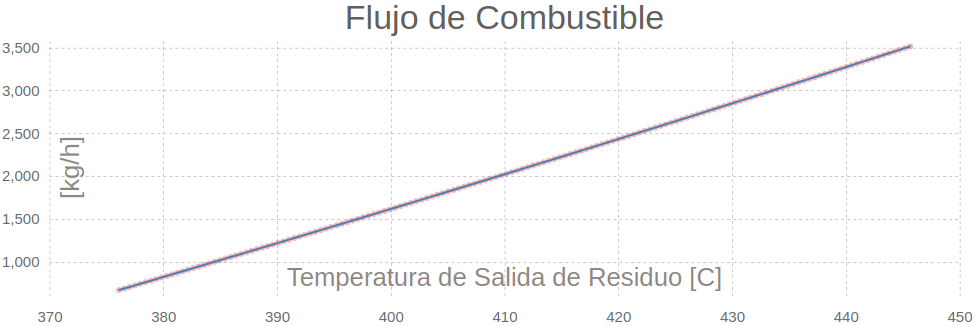
\includegraphics[scale=0.46]{images/graph-t_out-fuel}
\caption[Flujo de combustible en función de Temperatura de salida de residuo]{Flujo de combustible en función de la temperatura de salida de residuo.}
\label{fig:graph-t_out-fuel}\end{center}\end{figure}
\par Este comportamiento corresponde a que el combustible es la fuente de calor del horno y cualquier necesidad de energía adicional en el proceso requiere mayor flujo de combustible. Este comportamiento también se observa al aumentar el flujo de la carga, la humedad relativa y el exceso de aire, de forma independiente.
\par Al aumentar el flujo de combustible por el requerimiento de una temperatura de salida del fluido mayor, y manteniendo el resto de las variables de entrada, como exceso de aire y humedad relativa fijas, se nota un aumento en la temperatura de arco radiante (Fig. \ref{fig:graph-t_out-arc}) y, por consecuencia, en la temperatura de salida de los gases de chimenea (Fig. \ref{fig:graph-t_out-chim}).
\begin{figure}[H]\begin{center}
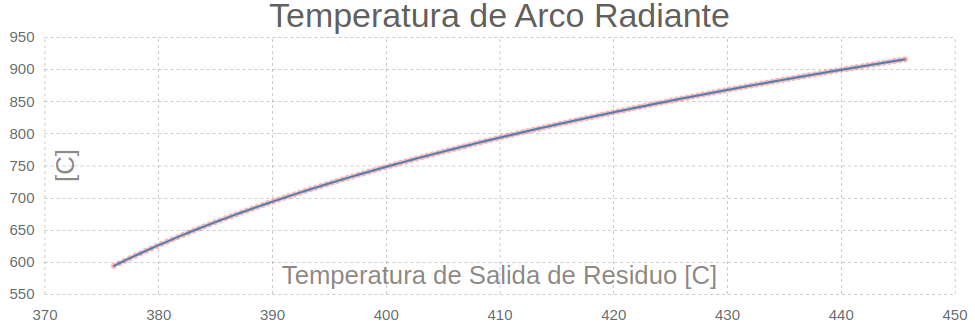
\includegraphics[scale=0.46]{images/graph-t_out-arc}
\caption[Temperatura de arco radiante en función de Temperatura de salida de residuo]{Temperatura de arco radiante en función de la temperatura de salida de residuo.}
\label{fig:graph-t_out-arc}\end{center}\end{figure}
\par El aumento observado en las Figuras \ref{fig:graph-t_out-fuel} y \ref{fig:graph-t_out-chim} se traduce en mas energía y gases de combustión liberados al ambiente, disminuyendo la eficiencia del horno y aumentado la contaminación generada por el proceso.
\begin{figure}[H]\begin{center}
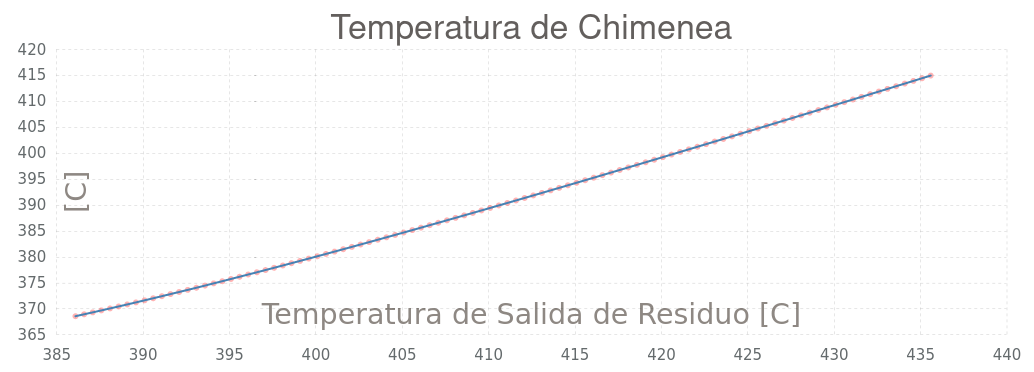
\includegraphics[scale=0.46]{images/graph-t_out-chim}
\caption[Temperatura de chimenea en función de Temperatura de salida de residuo]{Temperatura de chimenea en función de la temperatura de salida de residuo.}
\label{fig:graph-t_out-chim}\end{center}\end{figure}
\par Para la variable de la relación de calor absorbido por zona, la tendencia observada en la Figura \ref{fig:graph-t_out-dist} es decreciente, lo que se traduce en que el porcentaje de la absorción de calor disminuye en la zona radiante y aumenta en la zona convectiva, a pesar de que el calor transferido es siempre mayor en la zona radiante se debe considerar que están aumentando las pérdidas de calor por la chimenea.
\begin{figure}[H] \begin{center}
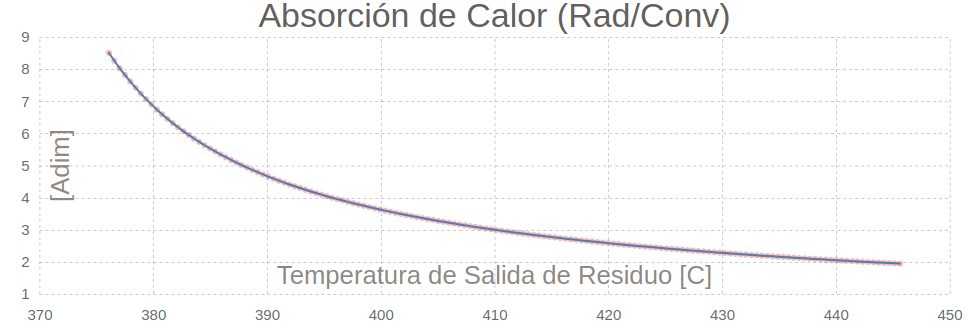
\includegraphics[scale=0.46]{images/graph-t_out-dist}
\caption[Distribución de absorción de calor en función de Temperatura de salida de residuo]{Tasa de distribución de absorción de calor entre zona radiante y convectiva en función de la temperatura de salida de residuo.}
\label{fig:graph-t_out-dist} \end{center} \end{figure}
\par Ambas zonas transfieren mayor cantidad de calor al fluido, pero la zona convectiva refleja un aumento porcentual mayor, proporcional a la temperatura de los gases de combustión, un factor a considerar es que la zona convectiva tiene un área de contacto casi diez veces mayor por la presencia de aletas.
\par La Figura \ref{fig:graph-t_out-efic} muestra la tendencia decreciente de la eficiencia térmica en función de la temperatura de salida del residuo. La tendencia refleja el incremento de las pérdidas de calor del horno como consecuencia de la menor absorción de calor en las secciones radiante y de escudo que no puede ser compensada por la sección convectiva. 
\begin{figure}[H]\begin{center}
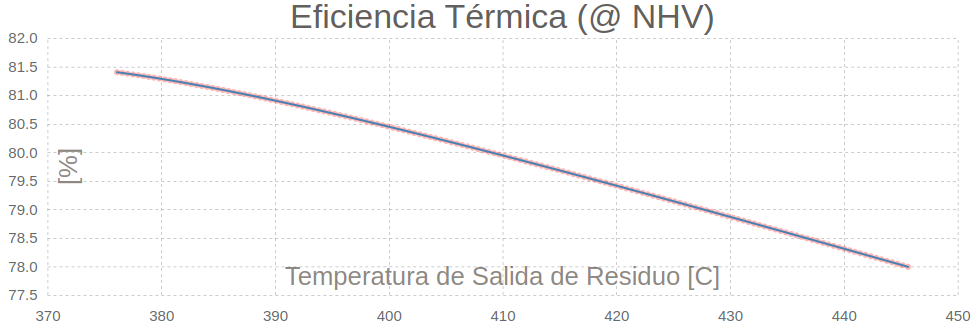
\includegraphics[scale=0.46]{images/graph-t_out-efic}
\caption[Eficiencia térmica en función de Temperatura de salida de residuo]{Eficiencia Térmica (@ Valor Calorífico Neto) en función de la temperatura de salida de residuo.}
\label{fig:graph-t_out-efic}\end{center}\end{figure}
\par Este comportamiento se observa también al aumentar las otras variables disponibles para este análisis, el exceso de aire, humedad y flujo de residuo, inversamente proporcional al aumento de la temperatura de los gases en la chimenea.
\par La Figura \ref{fig:graph-t_out-emi} muestra la tendencia ascendente de las emisiones de CO$_2$ con respecto a la temperatura de salida del residuo, lo cual, como ya se indicó, coincide con un mayor consumo de combustible y una disminución de la eficiencia térmica del horno.
\begin{figure}[H] \begin{center}
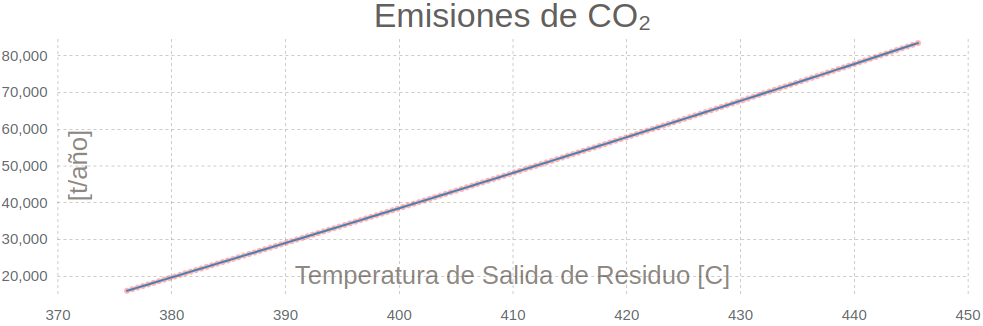
\includegraphics[scale=0.46]{images/graph-t_out-emi}
\caption[Emisiones de CO$_2$ en función de Temperatura de salida de residuo]{Emisiones de CO$_2$ en función de la temperatura de salida de residuo.}
\label{fig:graph-t_out-emi} \end{center} \end{figure}
\par Un comportamiento similar se observa para todas las variables estudiadas.

\subsection{Variación del exceso de aire y humedad relativa}
\par En la Figura \ref{fig:exceso-aire} se muestran las tendencias de las seis variables de salida en función al exceso de aire, agrupadas como se diseñó en el simulador, se observa el mismo comportamiento de aumento del flujo de combustible, temperatura de chimenea y emisiones de CO$_2$; y disminución de la eficiencia térmica y del porcentaje de absorción de calor en la zona radiante.
\par Observando que la única tendencia diferente es la correspondiente a la temperatura de arco radiante, que disminuye incluso al aumentar el flujo másico de los gases de combustión, a causa de que el calor generado ahora debe calentar una masa de aire adicional en la sección de radiación, como se aprecia en la ecuación \ref{eq:llama} de temperatura de arco radiante, descrita en la sección de combustión de hidrocarburos.
\begin{figure}[H] \begin{center} 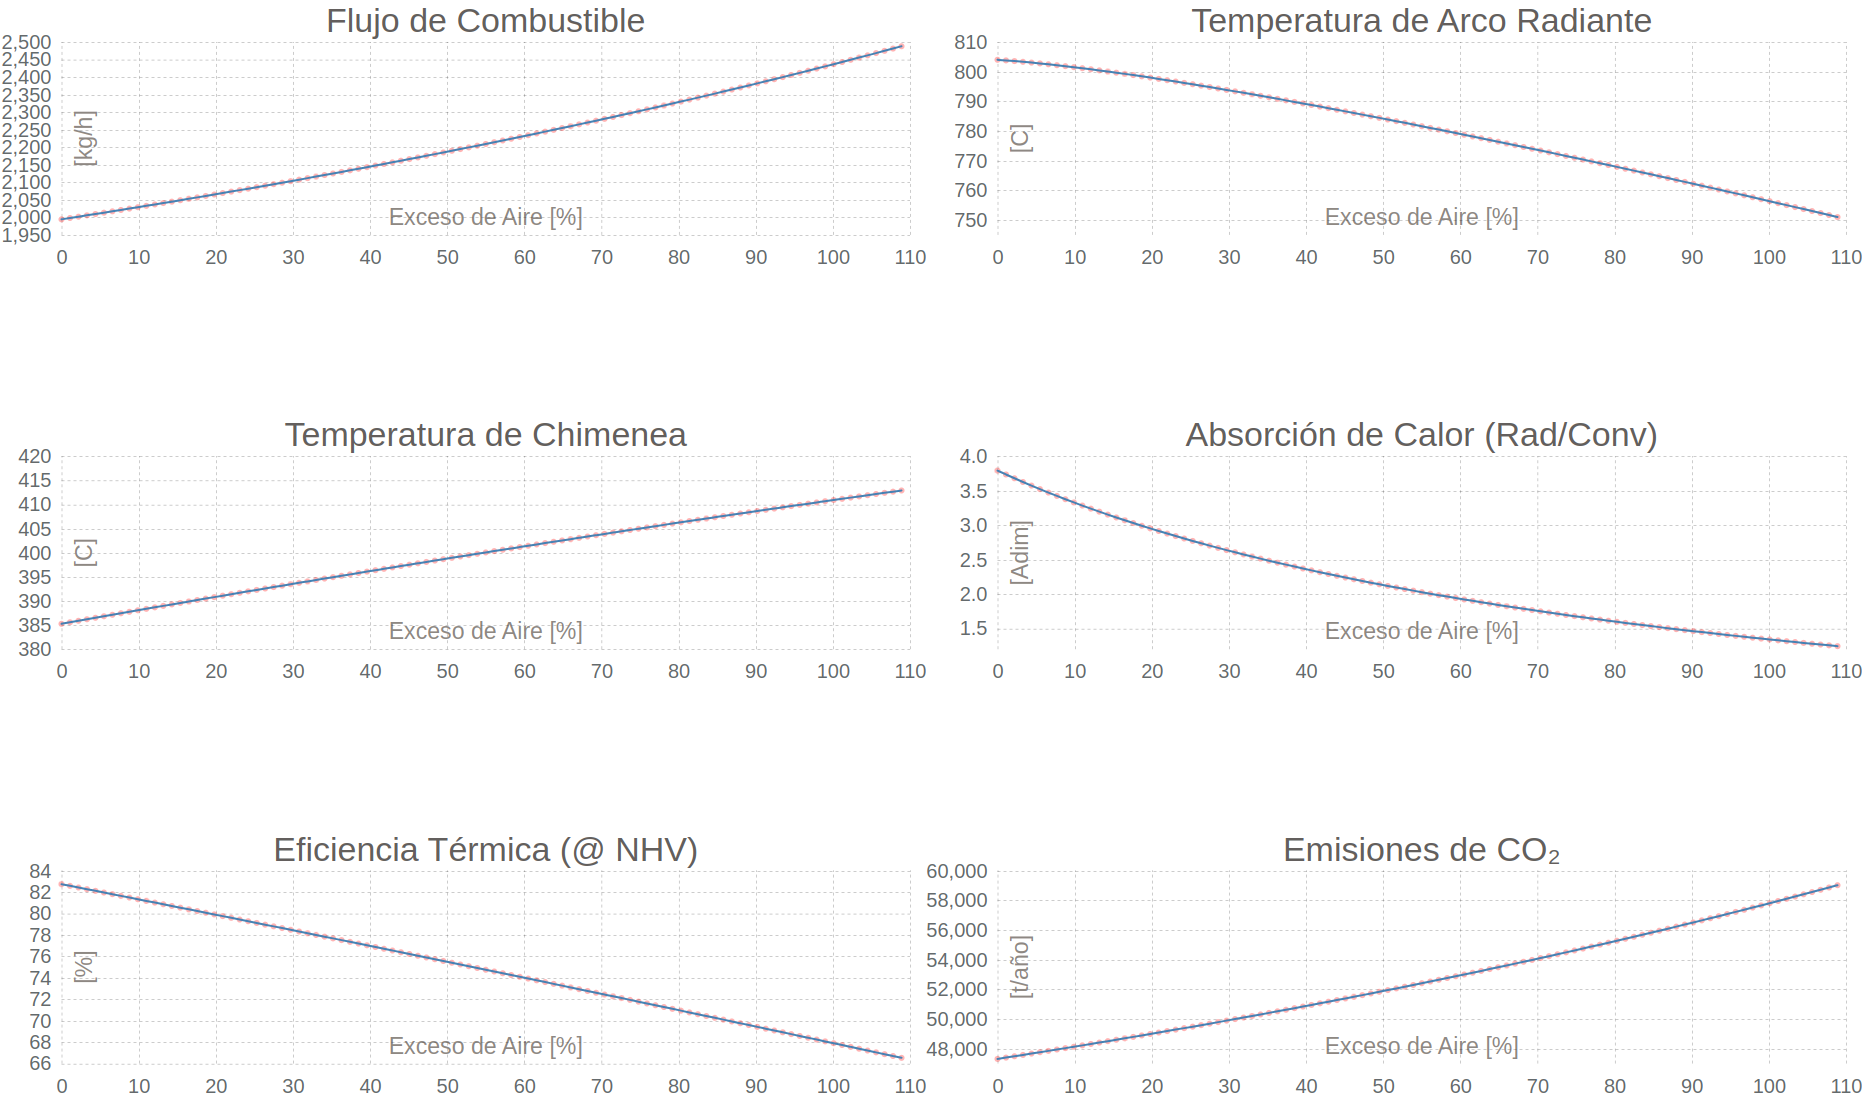
\includegraphics[scale=0.249]{images/exceso-aire}
\caption[Curvas de tendencia para la variación de exceso de aire]
{Curvas de tendencia para la variación de exceso de aire.}
\label{fig:exceso-aire} \end{center} \end{figure}
\par Comportamiento y tendencias similares se observan cuando se varia la humedad relativa en el aire de alimentación. Con lo que se tiene una referencia de la tendencia en todas las variables abiertas para graficar.

\section{Resultados del modo comparativo}
\par Este modo de la interfaz del simulador permite observar vis a vis los parámetros de dos condiciones de operación del horno, una condición Base y otra Modificada. Esta presentación posibilita comparar los cambios en las variables proceso y analizar las causas de los cambios registrados en los resultados operacionales.
\par En la Tabla \ref{tbl:comparison-cp} se observa un resumen de un caso Base, con las condiciones operacionales de diseño, y un caso Modificado en el cual el combustible (gas de refinería) contiene cuatro veces más hidrógeno, una menor proporción de hidrocarburos C1, C2 y C3, y, valores de poder calorífico ligeramente mayores.
\par La Tabla \ref{tbl:comparison-cp} contiene las condiciones operacionales del residuo atmosférico, los factores de ensuciamiento internos y externos de los tubos radiantes, del escudo y convectivos, las condiciones de combustión y la composición y las propiedades del combustible.
\begin{table}[H]
\caption{Condiciones de proceso del modo comparativo del simulador}
\label{tbl:comparison-cp} \centering \begin{tabular}{l|c|c}
\quad\quad\quad CASO    & BASE & MODIFICADO \\
\hline
\multicolumn{3}{c}{Residuo atmosférico} \\
Flujo volumétrico,  m$^3$/d   &14.309 &14.309 \\
Temperatura de entrada,  °C   &359    &359    \\
Temperatura de salida,  °C    &411    &411    \\
Gravedad específica           &0,84   &0,84   \\
Calor absorbido total,  MW    &20,862 &20,862 \\
\hline
\multicolumn{3}{c}{Factores de ensuciamiento} \\
Rfi (interno) radiante,  m$^2$-K/W 10$^{-3}$        &0,100  &0,100 \\
Rfi interno escudo/convectivo,  m$^2$-K/W 10$^{-3}$ &0,100  &0,100 \\
Rfo externo escudo/convectivo,  m$^2$-K/W 10$^{-3}$ &0,100  &0,100 \\
\hline
\multicolumn{3}{c}{Condiciones de combustión} \\
Exceso de aire, \%                      &20     &20   \\
Temperatura del aire de combustión, °C  &27     &27   \\
Humedad relativa, \%                    &50     &50   \\
Humedad del aire,  gH$_2$O/kg aire seco &11,107 &11,107\\
Pérdidas de calor al ambiente, \%       &1,5    &1,5  \\
\hline
\multicolumn{3}{c}{Características del combustible} \\
Metano (CH$_4$), \%          &56,47  &30,47  \\
Etano (C$_2$H$_6$), \%       &15,15  &8,15   \\
Propano (C$_3$H$_8$), \%     &6,22   &5,22   \\
n-Butano (C$_4$H$_{10}$), \% &1,76   &1,50   \\
i-Butano (C$_4$H$_{10}$), \% &0,75   &0,75   \\
Etileno (C$_2$H$_4$), \%     &1,58   &1,58   \\
Propileno (C$_3$H$_6$), \%   &2,77   &2,77   \\
Monóxido de carbono (CO), \% &0,66   &0,66   \\
Hidrógeno (H$_2$), \% &11,42&\colorbox{lightgray}{45,68}\\
Nitrógeno (N$_2$), \%        &0,68   &0,68   \\
Dióxido de carbono (CO$_2$), \%&2,54 &2,54   \\
\hline
Peso molecular,  kg/kmol               &21,149 &14,972 \\
Calor específico Cp (T comb),  kJ/kg-K &3,410  &7,595  \\
Poder Calorífico Neto (NCV),  kJ/kg    &45,718 &47,680 \\
Poder Calorífico Bruto (GCV),  kJ/kg   &50,268 &52,814 \\
\end{tabular}
\end{table}

\par En la Tabla \ref{tbl:comparison-r} se detallan uno a uno los resultados del caso Base y Modificado, de manera semejante a como se muestra en la interfaz web del simulador. Dentro de los resultados,vresaltan, la disminución del flujo de combustible en 3,5\% y, consecuentemente, de las emisiones de CO$_2$ en 10,8\%, lo que se debe directamente al incremento de la proporción de hidrógeno en el combustible para la operación modificada del horno, y, finalmente, el incremento de la eficiencia térmica.
\begin{table}[H]
\caption{Resultados del modo comparativo del simulador}
\label{tbl:comparison-r} \centering \begin{tabular}{l|c|c}
\quad\quad\quad CASO & BASE & MODIFICADO \\
\hline
\multicolumn{3}{c}{Flujos másicos,  kg/s} \\
Fluido de proceso (Residuo atmosférico)   &139,0         &139,0  \\
Combustible           &0,57 &\colorbox{lightgray}{0,55} \\
Aire                  &10,68         &10,38  \\
Gases de combustión   &11,28         &10,92  \\
\hline
(A/C) Masa BH        &18,693 &19,034 \\
(A/C) Volumen BH     &13,795 &9,944  \\
\hline
Suministro Térmico Combustible,  MW  &26,118 &25,999 \\
Suministro Térmico Total,  MW        &26,266 &26,169 \\
\hline
\multicolumn{3}{c}{Calor Absorbido,  MW}\\
Sección Radiante - (\%)  &13,099 - (62,79) &13,185 - (63,20)\\
Sección Escudo - (\%)    &3,311 - (15,87)  &3,313 - (15,88) \\
Sección Convectiva - (\%)&4,441 - (21,29)  &4,353 - (20,87) \\
\hline
Temperatura de pared (tubos radiantes), °C &434  &434  \\
Temperatura de Arco radiante, °C         &798  &798  \\
Temperatura de Chimenea, °C              &391  &391  \\
Temperatura Máxima Aletas (perímetro), °C &377  &376  \\
\hline
\multicolumn{3}{c}{Análisis de gases de combustión (Base Húmeda)}\\
CO$_2$, \%     &8,72    &7,93    \\
N$_2$, \%      &71,84   &71,23   \\
O$_2$, \%      &3,17    &3,14    \\
H$_2$O, \%     &16,27   &17,70   \\
\hline
Emisiones de CO$_2$, tonelada/año &48.790  &\colorbox{lightgray}{43.523} \\
\hline
\multicolumn{3}{c}{Pérdidas de calor,  MW}\\
Por chimenea - (\% del total)&4,888 - (18,61) &4,796 - (18,33) \\
Al ambiente - (\% del total) &0,392 - (1,49)  &0,390 - (1,49) \\
\hline
Eficiencia Térmica @ NHV, \%  &79,90 &80,18 \\
%Eficiencia Térmica @ GHV, \%  &72,70 &72,43 \\
\end{tabular} \end{table}
\par Esta comparación parte del supuesto de que el incremento del porcentaje de hidrógeno en el combustible puede ser manejado satisfactoriamente por los quemadores.

\par Otra comparación, resumida en la Tabla \ref{tbl:comparison-air}, al modificar únicamente el exceso de aire, de 20\% a 40\%, se observa: aumento en el consumo de combustible en 3,4\%, aumento en las emisiones de CO$_2$ en 3,6\%, aumento en el flujo de gases de combustión en 16,9\% y disminución en la eficiencia térmica de 2,9\%. 
\par Estos resultados se deben al consumo de energía térmica por parte del aire adicional suministrado al horno. Energía que no es transferida, subsiguientemente, al residuo atmosférico y que eventualmente se pierde por la chimenea. Evidenciando la importancia de esta variable en el proceso.
\begin{table}[H]
\caption{Resumen de comparación de aumento de exceso de aire en condiciones de diseño}
\label{tbl:comparison-air} \centering \begin{tabular}{l|c|c}
\quad\quad\quad CASO & BASE & MODIFICADO \\
\hline
\multicolumn{3}{c}{Condiciones de combustión} \\
Exceso de aire, \%      &20  &\colorbox{lightgray}{40}\\
Temperatura del aire de combustión, °C  &27     &27   \\
Humedad relativa, \%                    &50     &50   \\
Pérdidas de calor al ambiente, \%       &1,5    &1,5  \\
\multicolumn{3}{c}{Flujos másicos,  kg/s} \\
Fluido de proceso (Residuo atmosférico)   &139,0         &139,0  \\
Combustible           &0,57  &\colorbox{lightgray}{0,59} \\
Aire                  &10,68 & 12,93  \\
Gases de combustión   &11,28 &\colorbox{lightgray}{13,53}  \\
\hline
Exceso de oxígeno, \% (BH) &3,17   &5,50   \\
(A/C) Masa BH              &18,693 &21,809 \\
(A/C) Volumen BH           &13,795 &16,094  \\
\hline
Suministro Térmico Combustible,  MW  &26,118 &27,114 \\
\hline
Emisiones de CO$_2$, tonelada/año &48.790  &\colorbox{lightgray}{50.651} \\
\hline
\multicolumn{3}{c}{Pérdidas de calor,  MW}\\
Por chimenea - (\% del total)&4,888 - (18,61) &5,872 - (21,52) \\
Al ambiente - (\% del total) &0,392 - (1,49)  &0,407 - (1,49) \\
\hline
Eficiencia Térmica @ NHV, \%  &79,90 &\colorbox{lightgray}{76,99} \\
\end{tabular} \end{table}